\section{Movement Model}
A movement model describes how an entity moves through space given control input. It consists of internal parameters such as velocities and accelerations. Control input could be a direction of movement supplied by a human using a gamepad, or longer paths supplied by a game engine AI system. We have not seen any formal description of the movement model. Ususally some ad hoc newtonian physics concepts are combined with springs and animation curves to control the system.

Figure \ref{fig:movement:model} illustrates the definitions and concepts of a movement model.
\begin{figure}
    \centering
    
\includegraphics[width=0.75\columnwidth]{img/temporary.png}
    \caption{\kenny{Make a data-flow illustration of how a movement model and its components work. A kind of box-figure model with arrows on, showing how actors and controls work?}.}
    \label{fig:movement:model}
\end{figure}
In the following we limit \kenny{without loss of generalization} the description to locomotion in the plane. We parameterize the movement model as 
\begin{equation}
    \label{eq:model:parameterization}
 \model \equiv 
 \left\{ \modes,\,\interpolators \right\}
\end{equation}
where $\modes \equiv \seq{ \mode_1, \ldots, \mode_n}$ is a set of locomotion modes and $\interpolators \equiv \seq{ \interpolator_1, \ldots, \interpolator_m}$ is a set of interpolates that describes the transition between locomotion modes.  A movement model defines the behaviour of an actor 
\begin{equation}
    \label{eq:actor:def}
    \actor 
    \equiv
    \seq{
        \blend, \pos, \dtpos, \ori ,\dtori 
        }
\end{equation}
where $\pos$ and $\ori$ describe position, orientation and their derivatives are $\dtpos$ and $\dtori$. \kenny{To make this more concrete one can for example think of $\pos$ as the planar 2D position of the character root position in the world and $\ori$ could be the world facing direction of the character given as an angle measure in the 2D world plane.} The contribution weights for different movement modes are given by the vector $\blend \equiv \begin{bmatrix}\weight_1 & \ldots & \weight_n \end{bmatrix}^T$ that contains the contribution weights $\weight_l$ for $l \in \modes$. We use the convention that $\norm{\blend}^2 = 1$ and remark that usually only a couple of modes will be active as in a transition between walking and running where 
\begin{equation}
    \label{eq:contribusion:weight:example}
    \weight_l \equiv
    \begin{cases}
    0.8 & \text{if $l$ is walking} \\
    0.2 & \text{if $l$ is running} \\
    0 & \text{otherwise}
    \end{cases}\,.
\end{equation}
An actor is moved with a control signal, as a concrete example this could defined as follows
\begin{equation}
    \label{eq:control:signal:def}
    \control \equiv \seq{
    \mode_c, \interp_c, \Delta{t}_c, \pos_c, \ori_c}
\end{equation}
where $\mode_c$ is the desired locomotion mode, $\interp_c$ is the interpolation weight \kenny{what is this? Not very clear how it is related to the $\weight_l$s} , $\Delta t_c$ is the time-step \kenny{what kind of time-step?}  and target position and orientation is given by $\pos_c$ and $\ori_c$ respectively.

The sparsity of the control signal illustrates an inherent uncertainty in character animation, as we are challenged to infer a detailed path of movement through often complex environments given a very limited disambiguation or hints to the desired trajectory \cite{holden.ea16}. We notice that a sampling of the immediate surroundings could potentially be added as part of the control signal as in \cite{holden.ea17}. 

A step of the actor state can be described by two separate functions.
\begin{subequations}
\begin{align}
    \left( \pos^*, \ori^* \right) &\leftarrow \sfunc( \actor, \modes, \control) \label{eq:step:kinematics}\\
    \left( \blend^*, \interp{}^* \right) &\leftarrow  \sfunc_{\blend}(
        \blend, \interp_c, \interpolators, \Delta{t}_c
        )\label{eq:step:animation}
\end{align}
\end{subequations}
\kenny{What does the star notation mean here? The optimal solution or? Should perhaps be stated explicitly?} 

For $\sfunc_{\vec \omega}$ to keep the transitions defined in $\Delta{t}_c$ updates, each $\interpolator\in\interpolators$ should define a mapping $\Delta{t} \rightarrow \Delta \interp$ which also describes the duration of that transition since $\interp=1$ implies a completed interpolation. Each individual $t$ can be modelled uniquely or in a unified approach, using animator supplied curves, Sigmoids, linear interpolation or even a neural network to capture more subtleties in the transitions. In the case of transitions that are interrupted, we simply freeze existing transitions, and perform the incoming transition as a weighted combination of multiple transitions as shown in Figure \ref{fig:frozen-transition}. 
\begin{figure}
    \centering
    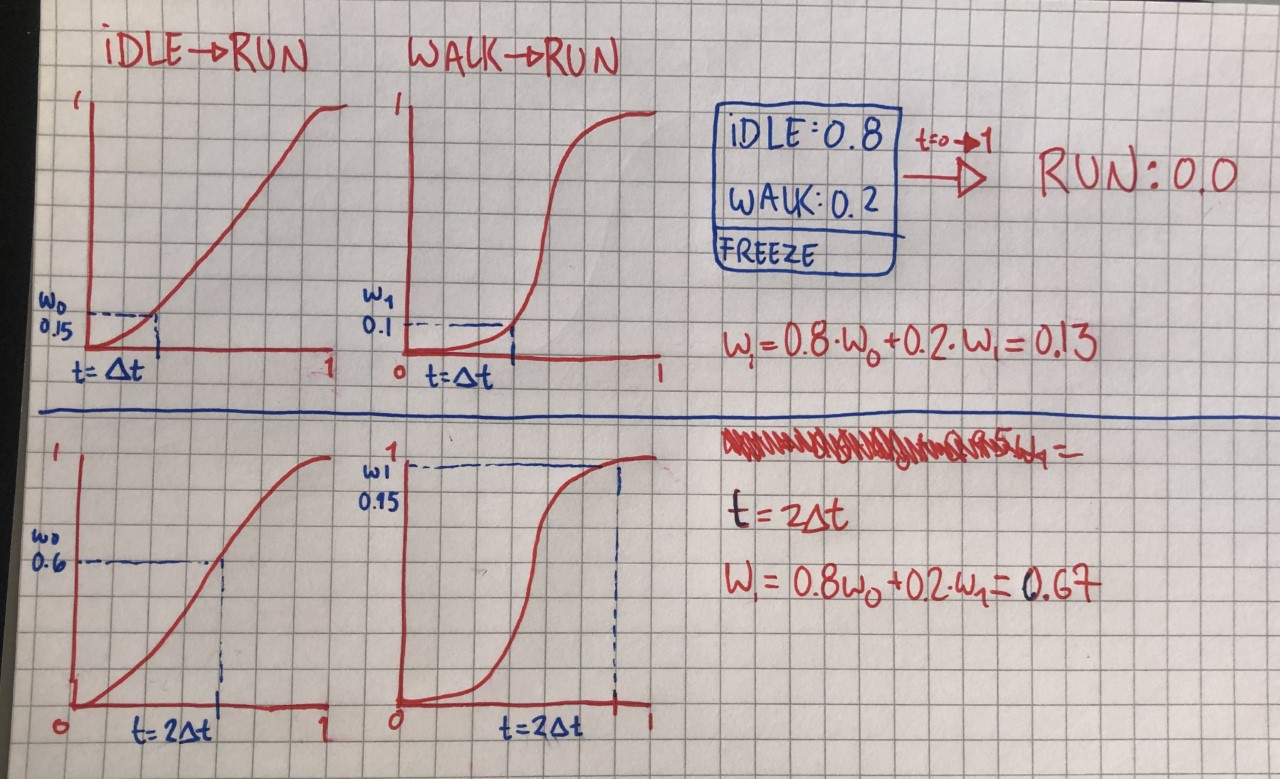
\includegraphics[width=0.75\columnwidth]{img/frozen-transitions}
    \caption{Frozen transition \kenny{Describe the take home message that reader should get from the figure}.}
  \label{fig:frozen-transition}
\end{figure}

By freezing and combining transitions in the case of interruptions, we are effectively approximating missing areas of the locomotion mode manifold by interpolations. This could be avoided by expanding $\interpolators$ to also contain transitions between combination of locomotion mode, or by expanding $\modes$ for a wider sampling of the manifold.

To evaluate $\sfunc$ we notice that each $\mode\in\modes$ should provide update routines $\dtpos_k^* \equiv \mode_{\pos,k}(\actor,\control)$ and $\dtori_k^* \equiv \mode_{\ori, k}(\actor,\control)$ which are then combined.
\begin{subequations}
\begin{align}
\dtpos^*&\leftarrow \sum_{k=1}^{m}\weight_k \,\mode_{\pos,k}(\actor,\control)\\
\dtori^*&\leftarrow \sum_{k=1}^{m}\weight_k \,\mode_{\ori,k}(\actor,\control)
\end{align}
\end{subequations}
\kenny{why sum over $m$ terms and not $n$ terms?}
The values can be inserted directly back into $\actor$ while $\pos$ and $\ori$ are updated with a forward Euler step \kenny{why this specific choice? why not just write: Position and orientation are time-integrated forward $\Delta t$ time,
\begin{subequations}
\begin{align}
    \pos^{t+\Delta t} &\leftarrow \pos^t + \int_{t}^{t+\Delta t} \dtpos^*\,dt \,, \label{eq:time:int:pos}\\
    \ori^{t+\Delta t} &\leftarrow \ori^t + \int_{t}^{t+\Delta t} \dtori^*\,dt\,, \label{eq:time:int:orientation}
\end{align}
\end{subequations}
where a simple forward Euler scheme suffices is our choice due to simplicity and performance.} using $\Delta{t}$. As before the update routines can be arbitrarily complex, which is natural given the idiosyncrasy of human movement. As such our choice of expressiveness in these function are imposing limits on the types of locomotion we are able to model. We use a simple yet expressive approach common to game development.   

velocity, velocity damper function, movement spring constant, orientation spring constant

velocity magnitude depends on the amount angular rotation. Slower when curving
move from current velocity to requested velocity is handled by spring.
move from orientation to requested orientation handled by soring.
Parameters are velocity, velocity damper function, velocity spring constant, orientation spring constant.


Notice that the formulation for $D$ is generic. In production a mapping between the generic movement model and a more context specific model would usually be needed. 

\subsection{missing}
Add animator constraint to model ? Example is 180. We dont start moving backwards immediately. First we rotate 90 degrees on the spot and then we start a 90 degree run to idle movement
Handle this by setting limits on rotation relative to forward movement ? Better to have a locomotion mode where velocity magnitude is 0 when facing relative to direction i < threshold.

Clear description of entire parameter set

Show very clear example. Pseudo code with idle and walk state. 



\section{Basic terminology}
Define animation database as $\mathcal{D}$

Define Movement model

Define Animation warping.


\section{Animation Warping}
We need a warping system that preserves ground truth. And some linear metric for divergence than can be scaled up from 0.


\section{Optimization Procedure}
We need some regularization to ill posed problem
\subsection{Primary movement modes}
Idea: Identify areas in the animations with cyclic movement for some duration. Cluster these segments into buckets with some threshold. We now have the velocity and number of main movement modes.
\subsection{Sparse user input}
If we allow extremely high frequency changes in the user input a wide variety of movement model configurations could follow the animation trajectory. We distribute sparse changes in user input over the animations, ie. few keypoints where we identify changes in the user input.


